\definecolor{slotcp}{RGB}{214,96,77}
\definecolor{slotzoom}{RGB}{67,147,195}
\definecolor{phblock}{RGB}{33,102,172}
\definecolor{phatt}{RGB}{230,145,56}
\definecolor{phagg}{RGB}{77,146,33}
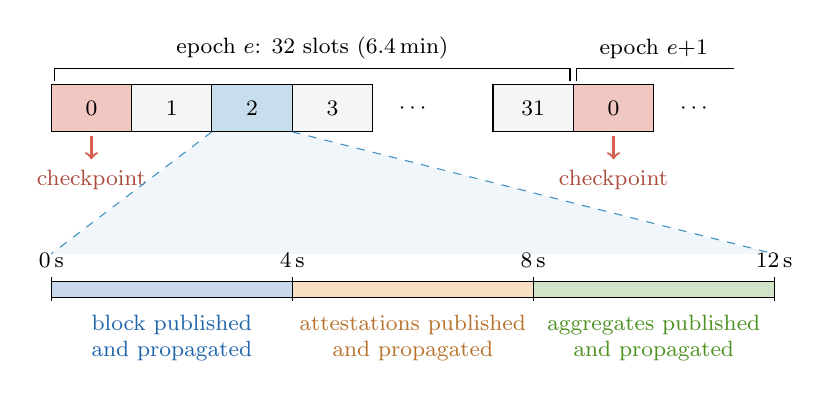
\begin{tikzpicture}[x=0.85cm,y=1cm,font=\footnotesize]
	% Zoom area, drawn first so it stays behind the labels
	\fill[slotzoom!8] (2.4,3) -- (0,1.45) -- (10.8,1.45) -- (3.6,3) -- cycle;
	% One epoch: 32 slots, a few of them drawn
	\draw[fill=slotcp!35] (0,3) rectangle ++(1.2,0.6);
	\node at (0.6,3.3) {0};
	\foreach \i/\lab in {1/1,3/3} {
		\draw[fill=gray!8] (\i*1.2,3) rectangle ++(1.2,0.6);
		\node at (\i*1.2+0.6,3.3) {\lab};
	}
	\draw[fill=slotzoom!30] (2.4,3) rectangle ++(1.2,0.6);
	\node at (3.0,3.3) {2};
	\node at (5.4,3.3) {$\cdots$};
	\draw[fill=gray!8] (6.6,3) rectangle ++(1.2,0.6);
	\node at (7.2,3.3) {31};
	\draw[fill=slotcp!35] (7.8,3) rectangle ++(1.2,0.6);
	\node at (8.4,3.3) {0};
	\node at (9.6,3.3) {$\cdots$};
	% Epoch brackets
	\draw (0.05,3.65) -- (0.05,3.8) -- (7.75,3.8) -- (7.75,3.65);
	\node[above] at (3.9,3.8) {epoch $e$: 32 slots ($6.4$\,min)};
	\draw (7.85,3.65) -- (7.85,3.8) -- (10.2,3.8);
	\node[above] at (9.0,3.8) {epoch $e{+}1$};
	% Checkpoints
	\draw[->,slotcp,thick] (0.6,2.95) -- ++(0,-0.3) node[below,text=slotcp!80!black] {checkpoint};
	\draw[->,slotcp,thick] (8.4,2.95) -- ++(0,-0.3) node[below,text=slotcp!80!black] {checkpoint};
	% Zoom on slot 2
	\draw[dashed,slotzoom] (2.4,3) -- (0,1.45);
	\draw[dashed,slotzoom] (3.6,3) -- (10.8,1.45);
	% Slot timeline, one colour per phase
	\fill[phblock!25] (0,0.9) rectangle (3.6,1.1);
	\fill[phatt!30]   (3.6,0.9) rectangle (7.2,1.1);
	\fill[phagg!25]   (7.2,0.9) rectangle (10.8,1.1);
	\draw (0,0.9) rectangle (10.8,1.1);
	\foreach \x/\t in {0/0\,s,3.6/4\,s,7.2/8\,s,10.8/12\,s} {
		\draw (\x,0.85) -- (\x,1.15);
		\node[above] at (\x,1.15) {\t};
	}
	\node[align=center,anchor=north,text=phblock] at (1.8,0.8) {block published\\and propagated};
	\node[align=center,anchor=north,text=phatt!80!black] at (5.4,0.8) {attestations published\\and propagated};
	\node[align=center,anchor=north,text=phagg] at (9.0,0.8) {aggregates published\\and propagated};
\end{tikzpicture}
